\subsection{Sensor Switch Attack}

The attack result differs from the two different controllers. In the classic
version after the attack it follows the path in clockwise direction after the
attack, in the improved version it follows the path in anticlockwise direction,
this can be explained looking at the angle of incidence of the robot when after
the attack return on the path.

\figref{fig:switchsensorattackresults} shows the comparison between the result
of the attack in the normal controller and in the improved controller.

\begin{figure}[htb]
	\centering
	\begin{subfigure}[b]{0.45\textwidth}
		\centering
		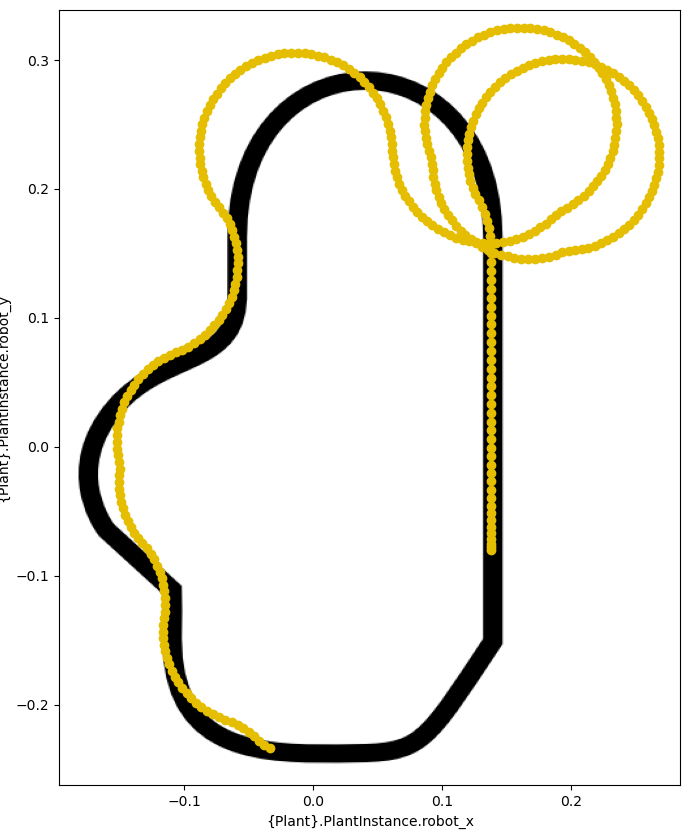
\includegraphics[width=\textwidth]{switch-sensors-attack}
		\caption{Line follower robot path when
		attacked into the normal controller}\label{fig:switchsenatt}
	\end{subfigure}
	\hfill
	\begin{subfigure}[b]{0.45\textwidth}
		\centering
		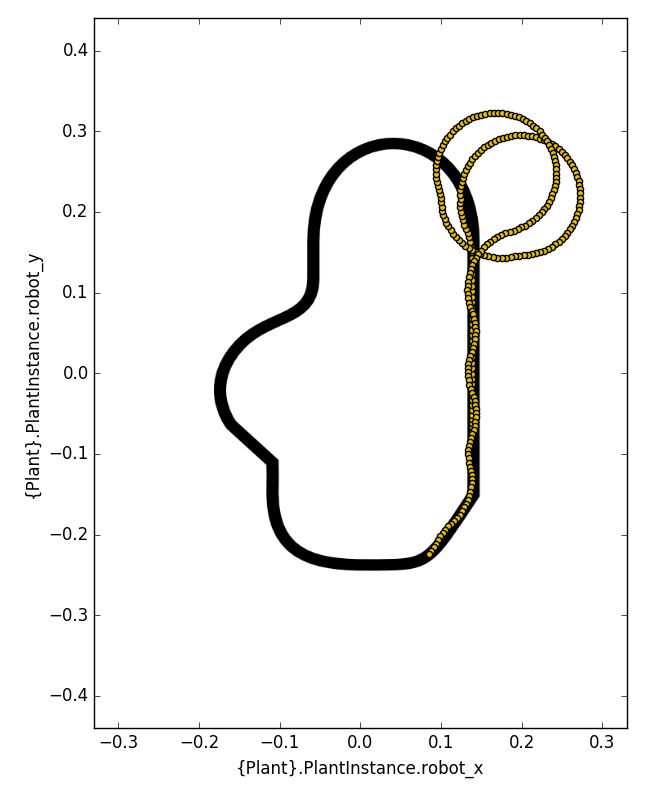
\includegraphics[width=\textwidth]{mm_switch_sensors_attack_improved}
		\caption{Line follower robot path when
		attacked into the improved controller}\label{fig:switchsenattim}
	\end{subfigure}
	\caption{Comparison between the normal and the improved controller in
	the Sensor Switch Attack}\label{fig:switchsensorattackresults}
\end{figure}
